\subsection{Súlyfüggvény kiszámítása}
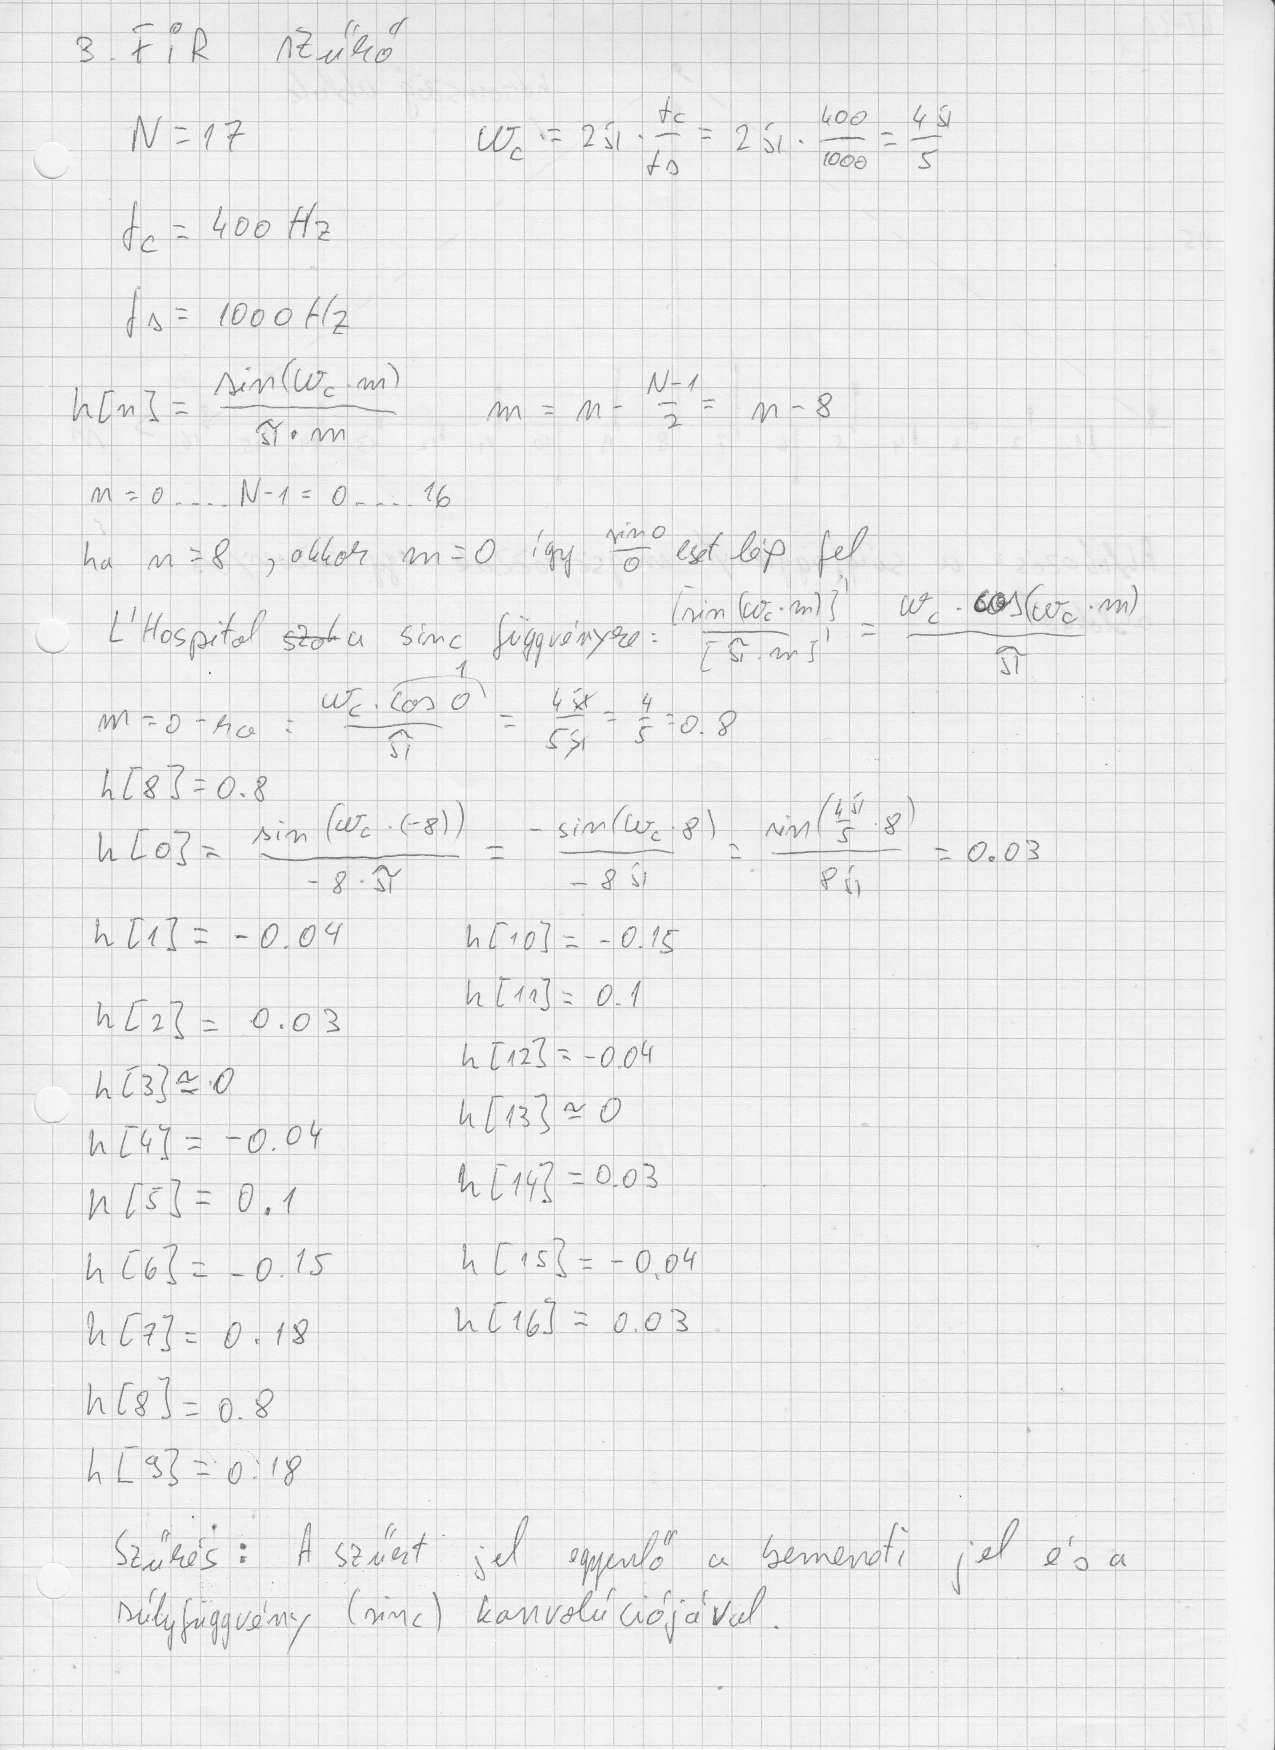
\includepdf[pages=-]{pdfs/fir.pdf}

\subsection{Python rész}

\subsubsection{Súlyfüggvény}

A következő ábrán látható a FIR szűrő súlyfüggvénye, a háromszög ablak és az ablakozás elvégzése utáni súlyfüggvény. Az ablakozás a súlyfüggvény beszorzása egy adott függvénnyel. Egyes típusú FIR szűrő, mivel páratlan a súlyfüggvény nem nulla elemeinek száma (N=17) és a súlyfüggvény szimmetrikus.

\begin{figure}[H]
    \centering
    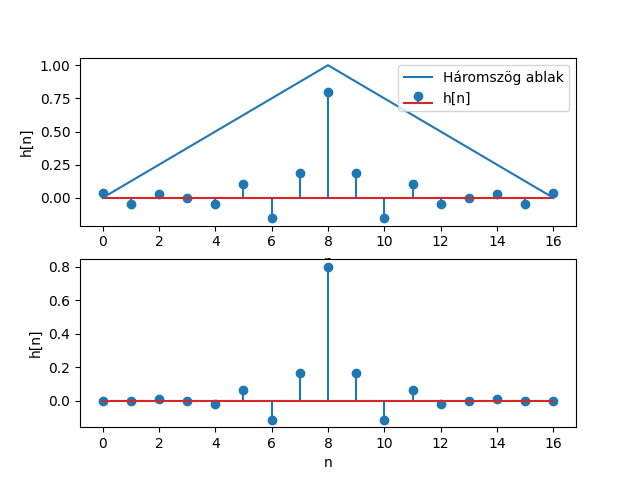
\includegraphics[scale=0.5]{figures/h.png}
    \caption{FIR súlyfüggvény, háromszög ablakkal}
\end{figure}

\subsubsection{Szűrés}

FIR szűrőnél a szűrt érték kiszámítható a bemeneti jel és a FIR súlyfüggvényének konvolúciójaként. Az alábbi ábrán látható egy 10 Hz-es és 470 Hz-es szinusz jel, ezek összege és a jel spektruma:

\begin{figure}[H]
    \centering
    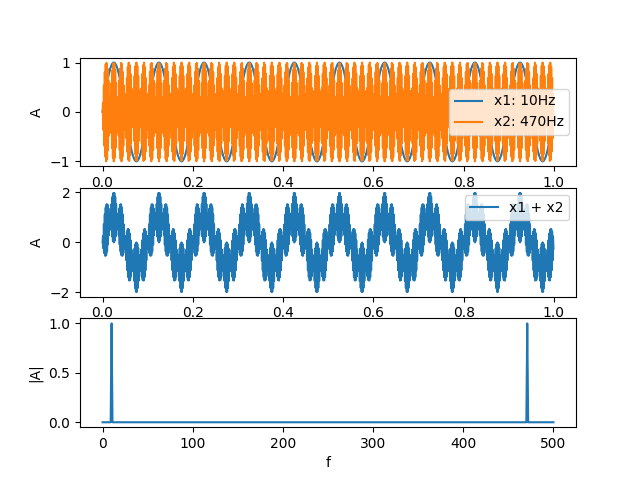
\includegraphics[scale=0.5]{figures/fir_sin.png}
    \caption{Bemeneti jel, két szinusz összege}
\end{figure}

A konvolúció elvégzése után a 470 Hz-es szinusz jelt ki sikerült szűrni: 

\begin{figure}[H]
    \centering
    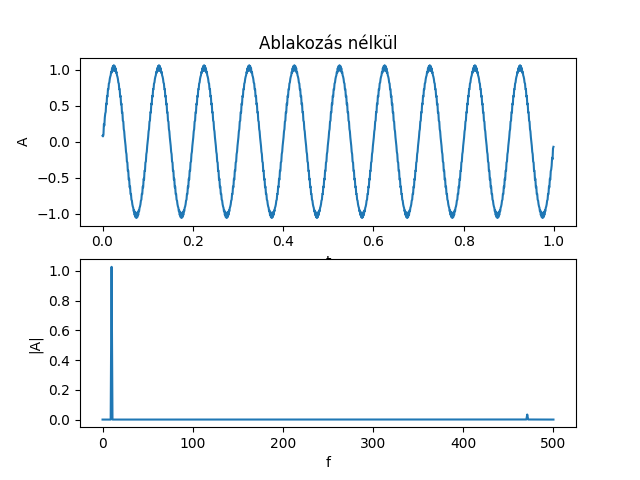
\includegraphics[scale=0.5]{figures/fir_no_win.png}
    \caption{Szűrés eredménye}
\end{figure}
